\documentclass{beamer}
\usepackage{tcolorbox}

%\beamerdefaultoverlayspecification{<+->}
\newcommand{\data}{\mathcal{D}}

\DeclareMathOperator*{\argmax}{arg\,max}
\DeclareMathOperator*{\argmin}{arg\,min}

\newcommand\Item[1][]{%
	\ifx\relax#1\relax  \item \else \item[#1] \fi
	\abovedisplayskip=0pt\abovedisplayshortskip=0pt~\vspace*{-\baselineskip}}
\usepackage{amsmath}
\usepackage{amssymb}


\usetheme{metropolis}           % Use metropolis theme


\title{Probabilistic View of Linear Regression}
\date{\today}
\author{Nipun Batra}
\institute{IIT Gandhinagar}
\begin{document}

\maketitle
\begin{frame}{Probabilistic View of Linear Regression}
\begin{itemize}[<+->]
\item  Example
function (black solid
diagonal line) and
its predictive
uncertainty at
x = 60 (drawn as a
Gaussian). 
    \begin{figure}[htp]
    \centering
    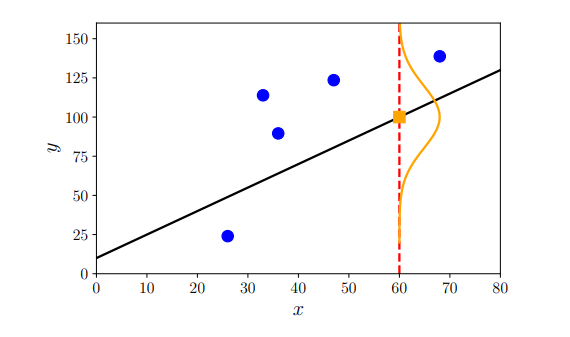
\includegraphics[width=8cm]{figures/probabilisticview.png}
    \caption{Probabilistic view of Linear Regression. Note that we don't have point estimates any longer.}
    \label{fig:prob1}
    \end{figure}
\end{itemize}
\end{frame}

\begin{frame}{Probabilistic View of Linear Regression}
\begin{itemize}[<+->]
\item  In this view, we consider a likelihood function
\begin{equation*}
p(y | \boldsymbol{x})=\mathcal{N}\left(y | f(\boldsymbol{x}), \sigma^{2}\right)
\end{equation*}
where $\boldsymbol{x} \in \mathbb{R}^{D}$ and the inputs and $y \in \mathbb{R}$ are the noisy function values, with the functional relationship between $\boldsymbol{x}$ and $y$ given by 
\begin{equation*}
y = f(\boldsymbol{x}) + \epsilon,
\end{equation*} where $\epsilon \stackrel{}{\sim} \mathcal{N}(0, \sigma^{2})$, is i.i.d. measurement noise with mean 0 and variance $\sigma^{2}$.

\end{itemize}
\end{frame}

\begin{frame}{Parameter Estimation and MLE}
\begin{itemize}[<+->]
\item  Suppose we are given a training set $\mathcal{D} := \{ (\boldsymbol{x}_1, y_1), (\boldsymbol{x}_2, y_2), \dots, (\boldsymbol{x}_n, y_N)$, consisting of $N$ inputs $\boldsymbol{x}_n \in \mathbb{R}^{D}$ and corresponding targets $y_n \in \mathbb{R}$, $n = 1, 2, 3, \dots N$. The graphical model for the same under the probabilistic viewpoint is as given below.
\begin{figure}[htp]
    \centering
    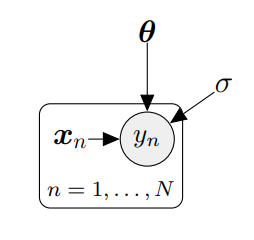
\includegraphics[width=2.7cm]{figures/graphicalmodel.png}
    \caption{Probabilistic Graphical Model for Linear Regression}
    \label{fig:pgmlr}
\end{figure}

In the above PGM, the observed random variables are shaded and the deterministic random variables are without circles.
\end{itemize}
\end{frame}


\begin{frame}{Parameter Estimation}
\begin{itemize}[<+->]
\item  Note that $y_i$ and $y_j$ are conditionally independent given their respective inputs $\boldsymbol{x}_i, \boldsymbol{x}_j$ so that the likelihood factorizes according to 
\begin{equation*}
\begin{aligned}
p(\mathcal{Y} | \mathcal{X}, \boldsymbol{\theta}) &=p\left(y_{1}, \ldots, y_{N} | \boldsymbol{x}_{1}, \ldots, \boldsymbol{x}_{N}, \boldsymbol{\theta}\right) \\
&=\prod_{n=1}^{N} p\left(y_{n} | \boldsymbol{x}_{n}, \boldsymbol{\theta}\right)=\prod_{n=1}^{N} \mathcal{N}\left(y_{n} | \boldsymbol{x}_{n}^{\top} \boldsymbol{\theta}, \sigma^{2}\right)
\end{aligned}
\end{equation*}
where $\mathcal{X}:= \{ \boldsymbol{x}_1, \boldsymbol{x}_2, \dots, \boldsymbol{x}_n \}$ and   $\mathcal{Y}:= \{ y_1, y_2, \dots, y_n \}$.
\item The likelihood and the factors $p(y_n | \boldsymbol{x}_n, \boldsymbol{\theta})$ are Gaussian due to the noise distribution.
\end{itemize}
\end{frame}

\begin{frame}{Parameter Estimation}
\begin{itemize}[<+->]
\item Note that once we have the optimal parameters $\boldsymbol{\theta}^{*} \in \mathbb{R}^{D}$, we can predict function values using this parameter estimate. For an arbitrary test input $\boldsymbol{x}_{*}$ the corresponding distribution of $y_{*}$ then becomes the following:
\begin{equation*}
    p(y_{*}|\boldsymbol{x}_{*}, \boldsymbol{\theta}) = \mathcal{N}(y_{*} | \boldsymbol{x}_{*}^{\top}\boldsymbol{\theta}^{*}, \sigma^{2})
\end{equation*}
\end{itemize}
\end{frame}

\begin{frame}{Maximum Likelihood Estimate}
\begin{itemize}[<+->]
\item A typically widely used method to find the desired parameters $\boldsymbol{\theta}_{ML}$ is \textit{maximum likelihood estimation}, where we find the parameters that maximize the likelihood. 
\begin{equation*}
    \boldsymbol{\theta}_{ML} = \argmax_{\boldsymbol{\theta}} p(\mathcal{Y} | \mathcal{X, \boldsymbol{\theta}})
\end{equation*}
\item Important Remark: The likelihood $p(\boldsymbol{y}|\boldsymbol{x}, \boldsymbol{\theta})$ is not a probability distribution in $\boldsymbol{\theta}$. It is a function of $\boldsymbol{\theta}$ and need not integrate to 1. Note that we compute likelihood for a given $\mathcal{Y}$ and $\mathcal{X}$. When we write $p(\mathcal{Y} | \mathcal{X, \boldsymbol{\theta}})$, we are talking about the conditional distribution of $\mathcal{Y}$, given a fixed $\mathcal{X}$ and $\boldsymbol{\theta}$. In the case of likelihood, $\boldsymbol{\theta}$ is the variable.
\end{itemize}
\end{frame}

\begin{frame}{Motivation for the Log Transformation}
\begin{itemize}[<+->]
\item Typically differentiating products of functions is much more complex than differentiating the sums of functions.
\item When we want to maximize likelihood, we are trying to maximize the product of several probabilities. This can lead to numerical underflow. 
\item Since logarithm function is monotonic, maximizing the logarithm of a function is equivalent to maximizing the function. 
\end{itemize}
\end{frame}

\begin{frame}{Negative Log Likelihood}
\begin{itemize}[<+->]
\item To find the optimal parameters, we minimize the negative log-likelihood as follows
\begin{equation*}
-\log p(\mathcal{Y} | \mathcal{X}, \boldsymbol{\theta})=-\log \prod_{n=1}^{N} p\left(y_{n} | \boldsymbol{x}_{n}, \boldsymbol{\theta}\right)=-\sum_{n=1}^{N} \log p\left(y_{n} | \boldsymbol{x}_{n}, \boldsymbol{\theta}\right)
\end{equation*}
\item Since the likelihood is Gaussian, we have,
\begin{equation*}
\log p\left(y_{n} | \boldsymbol{x}_{n}, \boldsymbol{\theta}\right)=-\frac{1}{2 \sigma^{2}}\left(y_{n}-\boldsymbol{x}_{n}^{\top} \boldsymbol{\theta}\right)^{2}+\text { const }
\end{equation*}
where the constant is independent of $\boldsymbol{\theta}$. 
\end{itemize}
\end{frame}

\begin{frame}{Negative Log Likelihood}
\begin{itemize}
\item We therefore get negative log likelihood to be finally,
\begin{equation*}
\begin{aligned}
\mathcal{L}(\boldsymbol{\theta}) &:=\frac{1}{2 \sigma^{2}} \sum_{n=1}^{N}\left(y_{n}-\boldsymbol{x}_{n}^{\top} \boldsymbol{\theta}\right)^{2} \\
&=\frac{1}{2 \sigma^{2}}(\boldsymbol{y}-\boldsymbol{X} \boldsymbol{\theta})^{\top}(\boldsymbol{y}-\boldsymbol{X} \boldsymbol{\theta})=\frac{1}{2 \sigma^{2}}\|\boldsymbol{y}-\boldsymbol{X} \boldsymbol{\theta}\|^{2} 
\end{aligned}
\end{equation*}
and $\boldsymbol{X}:= [\boldsymbol{x}_1, \dots, \boldsymbol{x}_N] \in \mathbb{R}^{N \times D}$ and $\boldsymbol{y}:= [y_1, \dots, y_N]^{\top} \in \mathbb{R}^{N}$. 

\item Note that the $n^{th}$ row of $\boldsymbol{X}$ corresponds to training input $\boldsymbol{x}_n$. 
\item If we minimize the above quantity, we get, 
\begin{equation*}
    \boldsymbol{\theta}_{ML} = \big(\boldsymbol{X^{\top}X}^{-1}\big)\boldsymbol{X}^{\top}\boldsymbol{y}
\end{equation*}

 \end{itemize}
\end{frame}

\begin{frame}{Estimating the noise variance}
\begin{itemize}[<+->]
\item Assumption so far: Noise variance $\sigma^{2}$ was known.
\item Now :Relax this assumption and obtain a maximum likelihood estimator $\sigma^{2}_{ML}$ for the noise variance.
\item We use the same procedure as above: write down the log-likelihood, compute its derivative with respect to $\sigma^{2} > 0$, set it to 0 and obtain the needed estimate.
\item Final Result: 
\begin{equation*}
    \sigma_{ML}^{2} = \frac{1}{N}\sum_{n=1}^{N}(y_n - \boldsymbol{x}_n^{\top}\boldsymbol{\theta})^{2}
\end{equation*}
 \end{itemize}
\end{frame}

\begin{frame}{Maximum A Posteriori Estimation}
\begin{itemize}[<+->]
\item MLE is prone to overfitting.
\item Need to mitigate the effects of huge parameter values. How to do this?
\item Answer: We place a prior $p(\boldsymbol{\theta})$ on the parameters.
\item Example: Gaussian prior $p(\theta) = \mathcal{N}(0, 1)$ on a parameter which we expect to lie in the interval [-2, 2]. 
\item Once we have a dataset $\mathcal{X}, \mathcal{Y}$, instead of maximizing the likelihood, we seek parameters to maximize the posterior distribution $p(\boldsymbol{\theta}|\mathcal{X}, \mathcal{Y})$.
\end{itemize}
\end{frame}


\begin{frame}{Maximum A Posteriori Estimation}
\begin{itemize}[<+->]
\item From Bayes Theorem, we have 
\begin{equation*}
p(\boldsymbol{\theta} | \mathcal{X}, \mathcal{Y})=\frac{p(\mathcal{Y} | \mathcal{X}, \boldsymbol{\theta}) p(\boldsymbol{\theta})}{p(\mathcal{Y} | \mathcal{X})}
\end{equation*}
\item Use the prior distribution $\mathcal{N}(0, b^{2} I_{n})$
\item Draw covariance matrix
\end{itemize}


\end{frame}
\begin{frame}{Maximum A Posteriori Estimation}
\begin{itemize}[<+->]
\item To find the MAP estimate, we follow the same steps as for MLE, firstly by considerating the log-posterior.
\begin{equation*}
    \log p(\boldsymbol{\theta} | \mathcal{X, Y}) = \log p(\mathcal{Y | X}, \boldsymbol{\theta}) + \log p(\boldsymbol{\theta}) + \text{ const }
\end{equation*}
\item We now minimze the negative log-posterior with respect to $\boldsymbol{\theta}$ to find $\boldsymbol{\theta}_{MAP}$
\item We have, 
\begin{equation*}
\boldsymbol{\theta}_{\mathrm{MAP}} \in \arg \min _{\boldsymbol{\theta}}\{-\log p(\mathcal{Y} | \mathcal { X }, \boldsymbol{\theta})-\log p(\boldsymbol{\theta})\}
\end{equation*}
\end{itemize}


\end{frame}

\begin{frame}{Maximum A Posteriori Estimation}
\begin{itemize}[<+->]
\item We have 
\begin{equation*}
\boldsymbol{\theta}_{\mathrm{MAP}} \in \arg \min _{\boldsymbol{\theta}}\{-\log p(\mathcal{Y} | \mathcal { X }, \boldsymbol{\theta})-\log p(\boldsymbol{\theta})\}
\end{equation*}
\item Now computing the gradient with respect to $\boldsymbol{\theta}$, we have 
\begin{equation*}
-\frac{\mathrm{d} \log p(\boldsymbol{\theta} | \mathcal{X}, \mathcal{Y})}{\mathrm{d} \boldsymbol{\theta}}=-\frac{\mathrm{d} \log p(\mathcal{Y} | \mathcal{X}, \boldsymbol{\theta})}{\mathrm{d} \boldsymbol{\theta}}-\frac{\mathrm{d} \log p(\boldsymbol{\theta})}{\mathrm{d} \boldsymbol{\theta}}
\end{equation*}
\item Using the conjugate Gaussian Prior $p(\boldsymbol{\theta}) = \mathcal{N}(\boldsymbol{0}, b^{2}\boldsymbol{I})$ on the parameters $\boldsymbol{\theta}$, we get the negative log posterior as follows:
\begin{equation*}
-\log p(\boldsymbol{\theta} | \mathcal{X}, \mathcal{Y})=\frac{1}{2 \sigma^{2}}(\boldsymbol{y}-\boldsymbol{X} \boldsymbol{\theta})^{\top}(\boldsymbol{y}-\boldsymbol{X} \boldsymbol{\theta})+\frac{1}{2 b^{2}} \boldsymbol{\theta}^{\top} \boldsymbol{\theta}+\text { const }
\end{equation*}
\item If we minimize the above quanitity, we get,
\begin{equation*}
    \boldsymbol{\theta}_{MAP} = \big(\boldsymbol{X^{\top}X} + \frac{\sigma^{2}}{b^{2}}\boldsymbol{I}\big)^{-1}\boldsymbol{X}^{\top}\boldsymbol{y}
\end{equation*}
\end{itemize}


\end{frame}

\begin{frame}{Maximum A Posteriori Estimation}
\begin{itemize}[<+->]
    \item In the below example, we place a Gaussian prior $p(\boldsymbol{\theta}) = \mathcal{N}(\boldsymbol{0}, \boldsymbol{I})$ on the parameters $\boldsymbol{\theta}$ and determine the MAP estimates. For the lower order polynomial the effect of the prior is not as pronounced as it is in the case of the higher order polynomial and keeps the polynomial relatively smooth in the second case.

    \begin{figure}[htp]
    \centering
    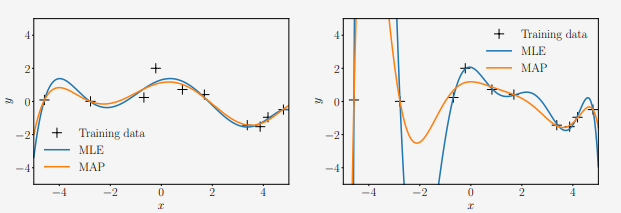
\includegraphics[width=8cm]{figures/map.png}
    \caption{Polynomial Regression and MAP Estimates. Degree 6 and 8 respectively for Figures (a) and (b).}
    \label{fig:map}
    \end{figure}

\end{itemize}
\end{frame}
\begin{frame}{Maximum A Posteriori Estimation}
\begin{itemize}[<+->]
    \item In the below example, we place a Gaussian prior $p(\boldsymbol{\theta}) = \mathcal{N}(\boldsymbol{0}, \boldsymbol{I})$ on the parameters $\boldsymbol{\theta}$ and determine the MAP estimates. For the lower order polynomial the effect of the prior is not as pronounced as it is in the case of the higher order polynomial and the prior keeps the second polynomial relatively smooth.

    \begin{figure}[htp]
    \centering
    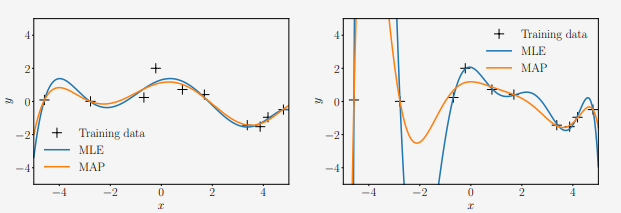
\includegraphics[width=8cm]{figures/map.png}
    \caption{Polynomial Regression and MAP Estimates. Degree 6 and 8 respectively for Figures (a) and (b).}
    \label{fig:map}
    \end{figure}

\end{itemize}
\end{frame}

\begin{frame}{Bayesian Linear Regression}
\begin{itemize}[<+->]
    \item In Bayesian Linear Regression, we consider the following model:
    \begin{equation*}
        \text{ Prior }: p(\boldsymbol{\theta}) = \mathcal{N}(\boldsymbol{m_{0}}, \boldsymbol{S}_{0})
    \end{equation*}
    \begin{equation*}
        \text{ Likelihood }: p(y | \boldsymbol{x}, \boldsymbol{\theta}) = \mathcal{N}(y | \boldsymbol{x}^{\top}\boldsymbol{\theta}, \sigma^{2})
    \end{equation*}
    \item As a PGM, we can represent it as follows:
        \begin{figure}[htp]
        \centering
        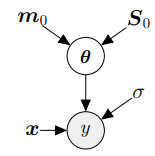
\includegraphics[width=2.5cm]{figures/blrpgm.png}
        \caption{Graphical Model for Bayesian Linear Regression}
        \label{fig:blrpgm}
    \end{figure}

\end{itemize}

\end{frame}



\begin{frame}{Bayesian Linear Regression}
\begin{itemize}[<+->]
\item The full probabilistic model, i.e., the joint distribution of observed and unobserved random variables, $y$ and $\boldsymbol{\theta}$, respectively, is
    \begin{equation*}
        p(y, \boldsymbol{\theta}|\boldsymbol{x}) = p(y|\boldsymbol{x, \theta})p(\boldsymbol{\theta})
    \end{equation*}
    

\item The posterior distribution in this case is given by,
\begin{equation*}
    p(\boldsymbol{\theta} | \mathcal{X}, \mathcal{Y})=\frac{p(\mathcal{Y} | \mathcal{X}, \boldsymbol{\theta}) p(\boldsymbol{\theta})}{p(\mathcal{Y} | \mathcal{X})}
\end{equation*}
\item The denominator above is called as the marginal likelihood or evidence, which ensures that the posterior is normalized and is independent of the parameters. An alternative way of writing the denominator is, 
\begin{equation*}
    p(\mathcal{Y | X}) = \int p(\mathcal{Y | X}, \boldsymbol{\theta})p(\boldsymbol{\theta})d\boldsymbol{\theta}
\end{equation*}
\end{itemize}
\end{frame}

\begin{frame}{Parameter Posterior}
\begin{itemize}[<+->]
\item The parameter posterior can be computed in closed form as follows:
\begin{equation*}
\begin{aligned}
p(\boldsymbol{\theta} | \mathcal{X}, \mathcal{Y}) &=\mathcal{N}\left(\boldsymbol{\theta} | \boldsymbol{m}_{N}, \boldsymbol{S}_{N}\right) \\
\boldsymbol{S}_{N} &=\left(\boldsymbol{S}_{0}^{-1}+\sigma^{-2} \mathbf{X}^{\top} \boldsymbol{X}\right)^{-1} \\
\boldsymbol{m}_{N} &=\boldsymbol{S}_{N}\left(\boldsymbol{S}_{0}^{-1} \boldsymbol{m}_{0}+\sigma^{-2} \boldsymbol{X}^{\top} \boldsymbol{y}\right)
\end{aligned}
\end{equation*}
\item The above posterior follows from:
\begin{equation*}
\begin{aligned}
&\text { Posterior } \quad p(\boldsymbol{\theta} | \mathcal{X}, \mathcal{Y})=\frac{p(\mathcal{Y} | \mathcal{X}, \boldsymbol{\theta}) p(\boldsymbol{\theta})}{p(\mathcal{Y} | \mathcal{X})}\\
&\text { Likelihood } \quad p(\mathcal{Y} | \mathcal{X}, \boldsymbol{\theta})=\mathcal{N}\left(\boldsymbol{y} | \boldsymbol{X} \boldsymbol{\theta}, \sigma^{2} \boldsymbol{I}\right)\\
&\text { Prior } \quad p(\boldsymbol{\theta})=\mathcal{N}\left(\boldsymbol{\theta} | \boldsymbol{m}_{0}, \boldsymbol{S}_{0}\right)
\end{aligned}
\end{equation*}
\end{itemize}
\end{frame}

\begin{frame}{Posterior Predictions}
\begin{itemize}[<+->]
\item The predictive distribution of $y_{*}$, at a test input $\boldsymbol{x}_{*}$ using the parameter prior $p(\boldsymbol{\theta})$ is computed as follows.

\begin{equation*}
\begin{aligned}
p\left(y_{*} | \mathcal{X}, \mathcal{Y}, \boldsymbol{x}_{*}\right) &=\int p\left(y_{*} | \boldsymbol{x}_{*}, \boldsymbol{\theta}\right) p(\boldsymbol{\theta} | \mathcal{X}, \mathcal{Y}) \mathrm{d} \boldsymbol{\theta} \\
&=\int \mathcal{N}\left(y_{*} | \boldsymbol{x}_{*}^{\top} \boldsymbol{\theta}, \sigma^{2}\right) \mathcal{N}\left(\boldsymbol{\theta} | \boldsymbol{m}_{N}, \boldsymbol{S}_{N}\right) \mathrm{d} \boldsymbol{\theta} \\
&=\mathcal{N}\left(y_{*} | \boldsymbol{x}_{*}^{\top} \boldsymbol{m}_{N}, \boldsymbol{x}_{*}^{\top} \boldsymbol{S}_{N} \boldsymbol{x}_{*}+\sigma^{2}\right)
\end{aligned}
\end{equation*}

\end{itemize}
\end{frame}

\begin{frame}{Bayesian Linear Regression Analysis}
% \begin{itemize}[<+->]

\begin{figure}[htp]
\centering
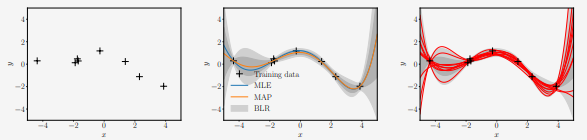
\includegraphics[width=11cm]{figures/blrfig1.png}
\caption{Bayesian linear regression and posterior over functions. (a) training data; (b) posterior distribution over functions; different shades correspond to different confidence intervals (c) Samples from the posterior over functions.}
\label{fig:blrfig1}
\end{figure}

% \end{itemize}
\end{frame}

\begin{frame}{Bayesian Linear Regression Analysis}
% \begin{itemize}[<+->]

\begin{figure}[htp]
\centering
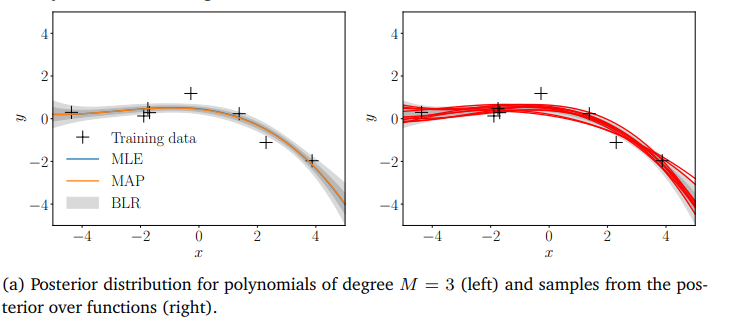
\includegraphics[width=7.5cm]{figures/blr21.png}
% \caption{Bayesian linear regression}
\label{fig:blrfig21}
\end{figure}
\begin{figure}[htp]
\centering
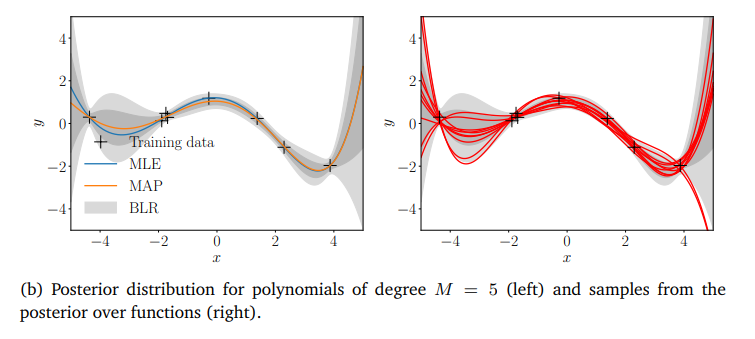
\includegraphics[width=8cm]{figures/blr22.png}
% \caption{Bayesian linear regression}
\label{fig:blrfig22}
\end{figure}

\end{frame}

\begin{frame}{Bayesian Linear Regression Analysis}
% \begin{itemize}[<+->]

\begin{figure}[htp]
\centering
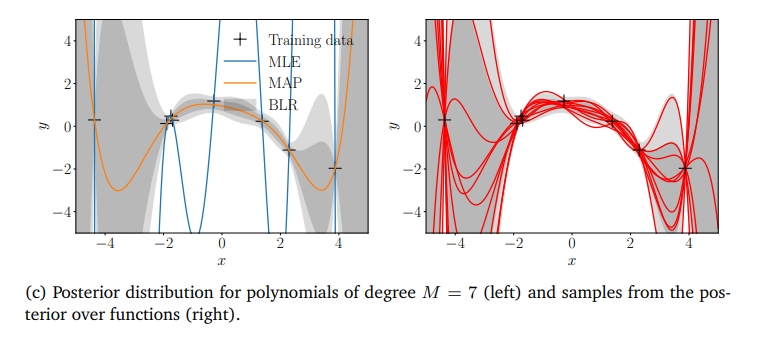
\includegraphics[width=7.5cm]{figures/blr23.png}
\caption{ Left
panels: The mean of the
Bayesian linear
regression model
coincides with the
MAP estimate. The
predictive
uncertainty is the
sum of the noise
term and the
posterior parameter
uncertainty, which
depends on the
location of the test
input. Right panels:
sampled functions
from the posterior
distribution.}
\label{fig:blrfig23}
\end{figure}

\end{frame}




\end{document}
